% !TEX root = ../main.tex
\chapter{Helium Rich Mass Transfer}\label{chap:he_mass_transfer}

\epigraph{We, all of us, are what happens when a primordial mixture of hydrogen and helium evolves for so long that it begins to ask where it came from.}{Jill Tarter}

\lettrine[lines=3]{A}s discussed in \autoref{sec:binary_evolution}, the presence of a companion measurably alters the evolution of a star. Typically this manifests as allowing matter to be exchanged between the components or the gravity of one star warping the photosphere of the other. In this chapter we focus on the first instance, where mass transfer occurs between two stars. We consider a binary system with \gls{zams} masses of \SI[parse-numbers=false]{30+10}{\msun}, and an initial period of $10^{0.6}\approx$ \SI{3.98}{\day}.

\section{Atypical abundance profiles}

Because the stars are quite close together and have a mass ratio of $\nicefrac{1}{3}$, when \gls{rlof} starts it is quite voracious, and becomes even more so during the contact phase. The donor star sheds its hydrogen-rich surface and material from the helium-rich core is exposed, which too becomes part of the accreted material. The material stream becomes increasingly helium-rich, depositing this material on top of a hydrogen-rich surface, causing the accretor to have an atypical abundance profile, as shown pictorally in \autoref{fig:composition_profile_evolution}. The net effect is that there is a helium-rich surface sitting atop a hydrogen-rich layer sitting atop a helium-rich core. At this stage thermohaline mixing is projected to occur, as there is an unstable composition gradient (owing to helium having a higher mean molecular weight than hydrogen).

\begin{table}
    \begin{subtable}[b]{0.49\linewidth}
        \centering
        \begin{tabular}{l|lr|rr|rr}
            \toprule
                                                                 &                              &                    &   \multicolumn{2}{c|}{Star 1}           &   \multicolumn{2}{c}{Star 2}           \\
                                                                 &                              &   \mlc{$t=0$\\(a)} &   \mlc{Begin\\(b)} &   \mlc{End\\(e)}   &   \mlc{Begin\\(c)} & \mlc{End\\(d)}    \\
            \midrule
             \multirow{5}{*}{\rotatebox[origin=c]{90}{Donor}}    & $M~/~\unit{\msun}$           &              30.00 &              27.93 &               7.56 &            26.91 &              17.43  \\
                                                                 & $R~/~\unit{\rsun}$           &               8.82 &              16.32 &              10.20 &            13.88 &               9.76  \\
                                                                 & $\log L~/~\unit{\lsun}$      &               5.07 &               5.30 &               5.25 &             5.16 &               4.94  \\
                                                                 & $X_\text{surf}$              &               0.70 &               0.70 &               0.09 &             0.70 &               0.57  \\
                                                                 & $Y_\text{surf}$              &               0.28 &               0.28 &               0.89 &             0.28 &               0.41  \\
             \midrule
             \multirow{5}{*}{\rotatebox[origin=c]{90}{Accretor}} & $M~/~\unit{\msun}$           &              10.00 &               9.99 &              20.97 &            11.00 &              14.57  \\
                                                                 & $R~/~\unit{\rsun}$           &               4.87 &               4.36 &               4.02 &             9.23 &               8.98  \\
                                                                 & $\log L~/~\unit{\lsun}$      &               3.73 &               3.81 &               4.89 &             4.90 &               5.06  \\
                                                                 & $X_\text{surf}$              &               0.70 &               0.70 &               0.09 &             0.70 &               0.57  \\
                                                                 & $Y_\text{surf}$              &               0.28 &               0.28 &               0.89 &             0.28 &               0.41  \\
             \midrule
             \multirow{3}{*}{\rotatebox[origin=c]{90}{Binary}}   & $P_\text{bin}~/~\unit{\day}$ &               3.98 &               3.85 &               4.41 &             3.14 &               2.52  \\
                                                                 & $a~/~\unit{\rsun}$           &              36.14 &              34.74 &              34.56 &            30.28 &              24.71  \\
                                                                 & Age~/~\unit{\kilo\year}      &               0.00 &            4707.16 &            6450.23 &          4712.75 &            4716.42  \\
             \bottomrule
        \end{tabular}
        \caption{Variable composition accretion}
        \label{tab:binary_configuration_parameters_variable_accretion}
    \end{subtable}%
    \begin{minipage}{0.1\linewidth}
    \phantom{a} % please
    \end{minipage}%
    \begin{subtable}[b]{0.49\linewidth}
        \centering
        \begin{tabular}{rr|rr}
             \toprule
                                                                                                                         \multicolumn{2}{c|}{Star 1}           &   \multicolumn{2}{c}{Star 2}            \\
                                                                                                                         \mlc{Begin\\(b)} &   \mlc{End\\(e)}   &   \mlc{Begin\\(c)} & \mlc{End\\(d)}     \\
             \midrule
                                                                                                                                    27.93 &               7.57 &              26.91 &              17.27 \\
                                                                                                                                    16.32 &              10.15 &              13.88 &               9.77 \\
                                                                                                                                     5.30 &               5.25 &               5.16 &               4.98 \\
                                                                                                                                     0.70 &               0.09 &               0.70 &               0.57 \\
                                                                                                                                     0.28 &               0.89 &               0.28 &               0.42 \\
             \midrule
                                                                                                                                     9.99 &              20.77 &              11.00 &              14.52 \\
                                                                                                                                     4.36 &               6.53 &               9.23 &               9.02 \\
                                                                                                                                     3.81 &               4.73 &               4.90 &               4.95 \\
                                                                                                                                     0.70 &               0.70 &               0.70 &               0.70 \\
                                                                                                                                     0.28 &               0.28 &               0.28 &               0.28 \\
             \midrule
                                                                                                                                     3.85 &               4.38 &               3.14 &               2.54 \\
                                                                                                                                    34.74 &              34.33 &              30.28 &              24.78 \\
                                                                                                                                  4707.16 &            6448.11 &            4712.75 &            4716.70 \\
            \bottomrule
        \end{tabular}
        \caption{Non-variable accretion}
        \label{tab:binary_configuration_parameters_standard_accretion}
    \end{subtable}
    \caption{The key evolutionary parameters of both stars and the binary configuration at five critical points: the initial parameters, and the beginning and ends of both epochs of \gls{rlof}. All values are rounded to 2 decimal places. The letter in parentheses represents which segment of \autoref{fig:composition_profiles_stages} (for \autoref{tab:binary_configuration_parameters_variable_accretion}) or \autoref{fig:composition_profiles_stages_standard} (for \autoref{tab:binary_configuration_parameters_standard_accretion}) the abundances are given in.}
    \label{tab:binary_configuration_parameters}
\end{table}

\begin{figure}
    \centering
    \begin{subfigure}[t]{0.45\columnwidth}
        \centering
        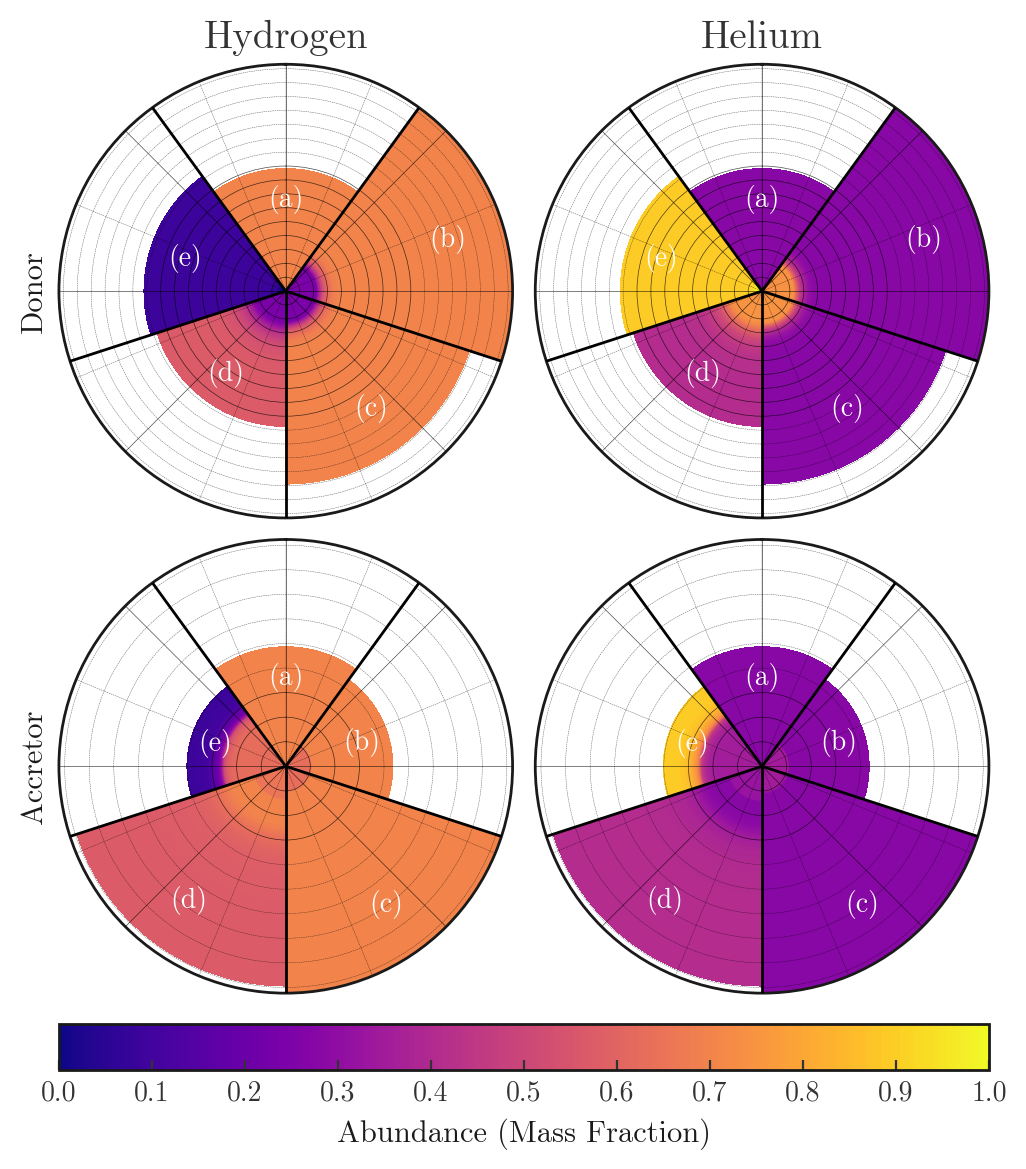
\includegraphics[width=\columnwidth]{images/HeliumRich/segmented_composition_profiles.png}
        \caption{Variable accretion} \label{fig:composition_profiles_stages}
    \end{subfigure}
    \begin{subfigure}[t]{0.45\columnwidth}
        \centering
        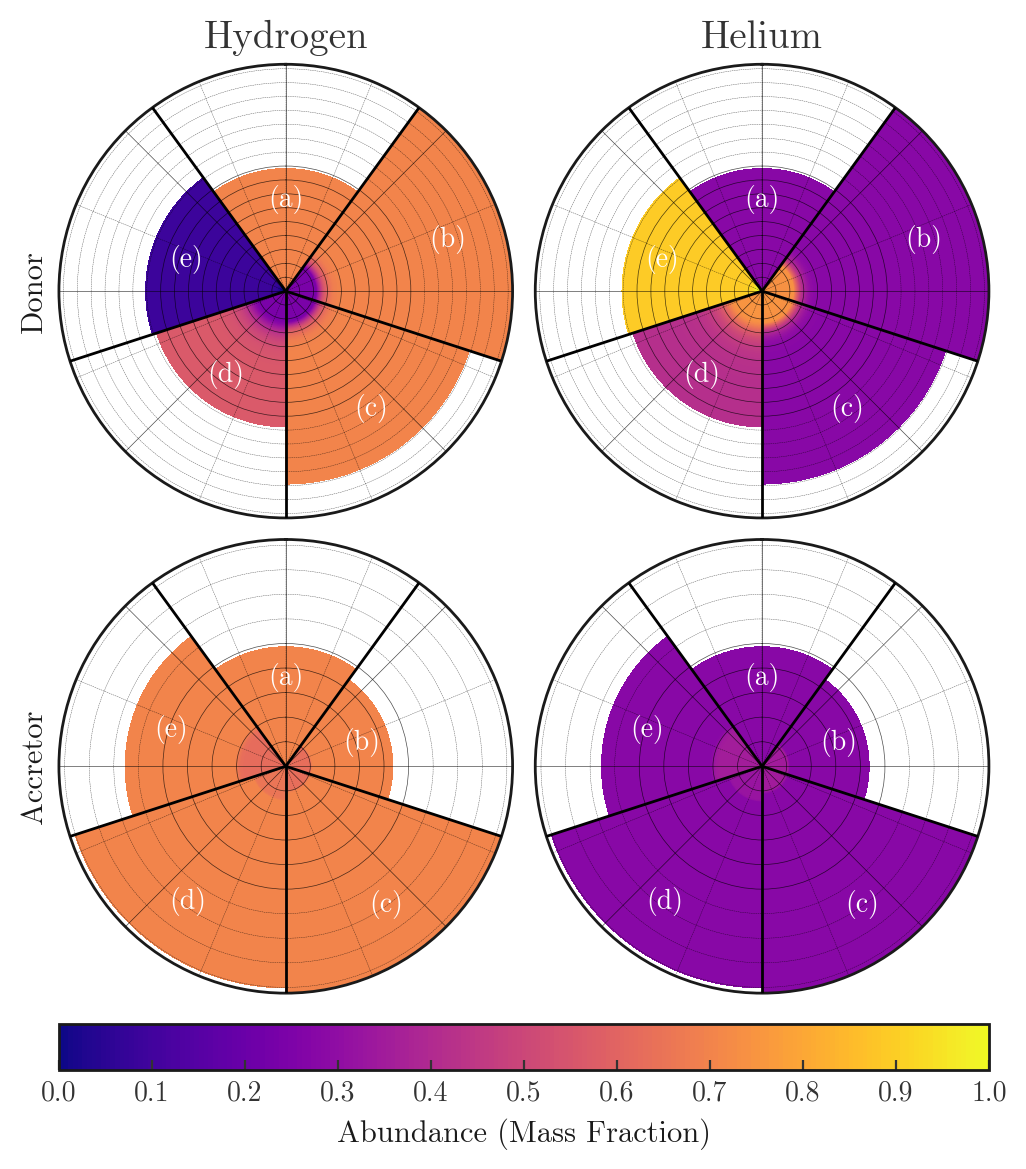
\includegraphics[width=\columnwidth]{images/HeliumRich/segmented_composition_profiles_STANDARD_BINARY.png}
        \caption{Non-variable accretion} \label{fig:composition_profiles_stages_standard}
    \end{subfigure}
    \caption[The chemical composition of each star as a function of the stellar radius for the donor and accretor at the five key stages of the binary's lifetime.]{The chemical composition of each star as a function of the stellar radius for the donor and accretor at the five key stages of the binary's lifetime as detailed in \autoref{tab:binary_configuration_parameters}. Letters are as given in the same table. Each grid marking in the radial direction represents \SI{1}{\rsun}.}
    \label{fig:composition_profile_evolution}%_eddington}
\end{figure}


\section{Comparison between variable and non-variable accretion}

In \autoref{fig:hrd_comparison_var_novarr} we display a comparative HR diagram between the cases of variable and non-variable accretion. In each case an \SI[parse-numbers=false]{30+10}{\msun} binary was evolved with the only difference between the two being whether material was allowed to have variable composition accretion or the standard accretion prescription. In the bottom panel only the companion is shown, as the donor has identical evolution in both cases.

The first and most striking conclusion that we can draw from this result is that the companion is, in the variable accretion case, hotter and more luminous than the non-variable case.

\begin{figure}[!htbp]
    \centering
    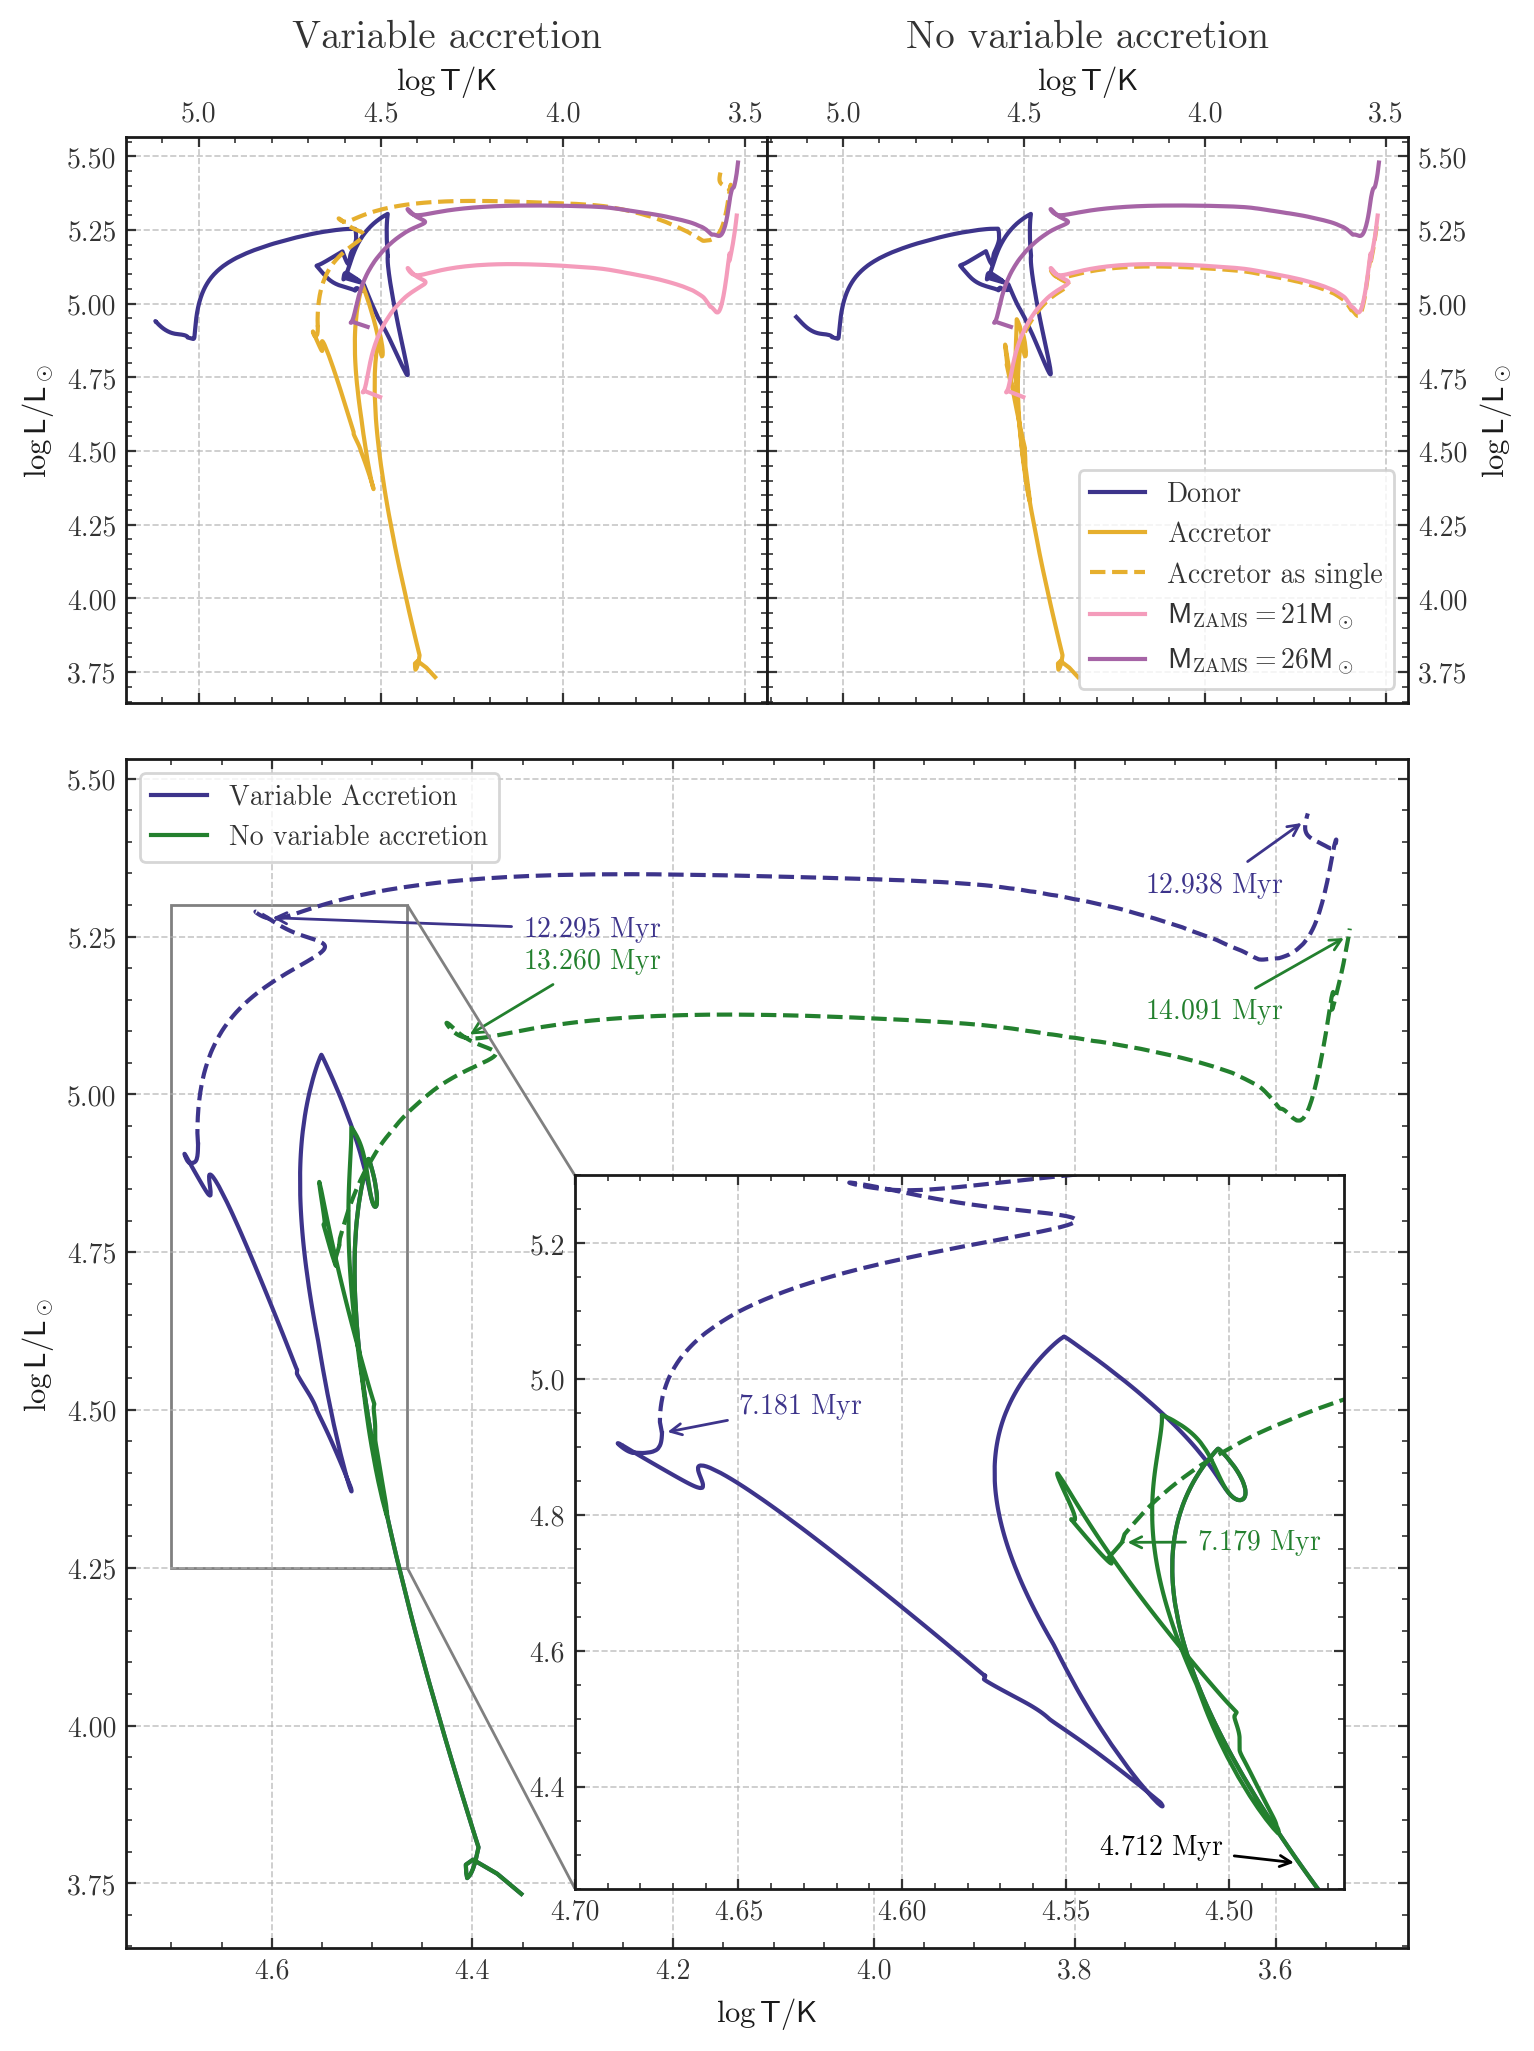
\includegraphics[width=0.8\textwidth]{images/HeliumRich/comparison_plot.png}
    \caption[An HR diagram showing the evolution of our model both with and without the variable accretion prescription.]{An HR diagram showing the evolution of our model both with (top left) and without (top right) the variable accretion prescription. The bottom panel shows only the evolution of the secondary. The point of divergence between the two models is shortly into the contact phase. The two dashed lines on the bottom HR diagram represent models evolved as the final model of the binary secondary, as a single star. On the top HR diagrams, the pink and brown models are single stars evolved with ZAMS masses of 21 and 26 \unit{\msun} respectively.}
    \label{fig:hrd_comparison_var_novarr}
\end{figure}

\section{Chapter Summary}